\documentclass[runningheads]{llncs}
\usepackage{graphicx}
\usepackage{doi}
\usepackage{xcolor}
\usepackage{caption}
\usepackage{amsmath}
\usepackage{multicol}

\newcommand\incomplete[1]{\textcolor{red}{#1}}

% Used for displaying a sample figure. If possible, figure files should
% be included in EPS format.
%
% If you use the hyperref package, please uncomment the following line
% to display URLs in blue roman font according to Springer's eBook style:
% \renewcommand\UrlFont{\color{blue}\rmfamily}

\begin{document}
%
\title{Highly Scalable Frontier-Led Chain Formations for Search and Exploration Problems}
\titlerunning{Highly Scalable Frontier-Led Chain Formations}

\author{Danny Roberts \and
Simos Gerasimou \and
Alan Millard}

\institute{
    Department of Computer Science,
    University of York, 
    York, UK
    \email{danny.roberts@york.ac.uk}\\
    \email{simos.gerasimou@york.ac.uk}\\
    \email{alan.millard@york.ac.uk}\\
}

\maketitle 

\begin{abstract}
Building upon the frontier-led swarming concept introduced by Tran\cite{tran2022}, this paper presents a novel adaptation that integrates a rigid chain formation with traditional flocking for the exploration and coverage of unknown environments. This approach augments Tran's method by guiding flocking dynamics into more structured outcomes through a rigid chain formation, maintaining the system's robustness to agent failure while achieving near-linear scalability. The agents in this system identify and maintain explicit links with their immediate neighbours, allowing for a more organized exploration strategy that complements the frontier-led approach. \incomplete{Summarize results here}. Future work will explore the capability of the chain to intelligently navigate around obstacles by splitting and reuniting, further solidifying this method's potential in applications such as humanitarian demining and ocean garbage clean-up. This research aims to offer a new perspective on the integration of rigid formations within swarm robotics, proposing a balanced approach between structured organization and the adaptive and scalable qualities of swarms.

\keywords{Swarm Robotics \and Scalability \and Formations}

\end{abstract}


\section{Introduction}
% Background & Context
Swarm intelligence, inspired by the collective behaviours of natural systems like colonies of ants and flocks of birds \cite{garnier2007}, aims to capture the powerful emergent behaviours that come with a system made up of simple agents\cite{mataric1995}.
Leveraging the principles of decentralized control and local interaction, swarm robotic systems offer unparalleled scalability, robustness, and flexibility, making them ideal for complex tasks ranging from environmental monitoring to search and rescue operations \cite{hamann2018,ijspeert2001}. 
Despite these advantages, challenges remain in maintaining effective communication and cohesive formations without prior knowledge of the terrain, a critical factor in the efficiency and success of swarm-based missions \cite{xu2014}. 
This research builds upon the foundation of "frontier-led swarming", introduced by Tran et al. \cite{tran2022}, to address these challenges through the novel integration of rigid chain formations, aiming to enhance both the structural integrity and scalability of swarm operations.

% Research Gap & objectives
    % Swarm dynamics COMBINED with rigid formation
    % obj: Enhanced scalability from formations that require leaders or central communication
    % Algorithms used etc.

% Paper structure
    % Just list the sections

% Simos introduction (full paper)
% Motivation - why do I care?
% Challenges - Why is this not already solved? (brief reference to related work)
% Despite ^^^, challenges remain unsolved; In this paper, we introduce _____
% Short summary of the results(?)
% List of key contribuions and paper structure

\section{Related Work}
\subsection{Swarm Algorithms}
    % Part 1 - Swarm algorithms, formations etc.

\subsection{Area coverage / search / exploration}
    % Part 2 - Non-swarm area coverage & formations


% ---=== Algorithm ===---

\section{Proposed Algorithm}
\subsection{Establishing the Basis}
Consider a set of $n$ agents $A^1, A^2...A^n$ where $p^i$ and $v^i$ represent the position and velocity of $A^i$.
We define a neighbour as another agent within a distance $d_x$ of the agent in question, with the set of all neighbours of $A^i$ represented by $N^i_x$:

\begin{equation}
    N^i_x = \{A^j \in A \setminus \{A^i\} : \|p^i - p^j\| \leq d_x\}
\end{equation}

\subsubsection{Flocking Forces}
At each time step $t$ a force is exerted on an agent based on the current state of its nearby neighbours. 
To implement Reynolds Boids \cite{reynolds1987}, we need the following forces per agent $A^i$. 
Each force has its own proximity radius $d_i$; e.g. $d_{coh}$ represents the cohesion radius.

\indent(\ref{eq:cohesion})\nobreakspace\textbf{Cohesion} 
    (pull towards the average position of its neighbours) \\
\indent(\ref{eq:alignment})\nobreakspace\textbf{Alignment} 
    (pull towards matching the velocity of its neighbours)\\
\indent(\ref{eq:separation})\nobreakspace\textbf{Separation} 
    (push away from neighbours that are too close).

\begin{equation}
    F^i_{coh} = (\frac{1}{|N^i_{\text{coh}}|} \sum_{j \in N^i_{\text{coh}}} p^j) - p^i \label{eq:cohesion}
\end{equation}
\begin{equation}
    F^i_{ali} = (\frac{1}{|N^i_{\text{ali}}|} \sum_{j \in N^i_{\text{ali}}} v^j) - v^i \label{eq:alignment}
\end{equation}
\begin{equation}
    F^i_{sep} = \sum_{j \in N^i_{sep}} \frac{p^i - p^j}{\|p^i - p^j\|^3} \label{eq:separation}
\end{equation}

\subsubsection{Goal Forces}
"Frontier-led Swarming" \cite{tran2022} combines basic flocking dynamics with a frontier generated from a local map.
This gives agents a goal in addition to maintaining the flock. 
Tran's work demonstrates an algorithm for generating this frontier cell, which we build on in our extension of their algorithm.
By subtracting an agent's current position from the fontier goal point $p^goal$, we can calculate a goal force $F_{goal}$ \ref{eq:goal} for each agent.

\begin{equation}
    F^i_{goal} = p^{goal} - p^i \label{eq:goal}
\end{equation}

\subsection{Chain formation}
The goal of a chain formation is to spread out across a frontier, such that the swarm as a whole can move in formation all covering new ground at once. In order to encourage spreading out in a line vs a cloud, we can apply a force to agents that are in front or behind of their peers. By using the dot product of an agent's velocity (or vector representing their heading) we get a value representing how far ahead or behind of an agent's heading its peer is. The average of these forces for all neighbours along with the other flocking forces will "flatten" a flock into a line or chain formation.

\begin{equation}
    F^i_{chn} = \frac{v^i}{|N^i_{\text{chn}}|} (\sum_{j \in N^i_{chn}} \hat{p^j} \cdot \hat{v^i})
\end{equation}


% We'll see if any of this is actually even needed to achieve the results we want

% \subsection{Explicit Partner Selection}
% Once an agent is in a chain-like arrangement it will attempt to select partners for its 

% \subsection{Propagation}
% When a robot is in a satisfactory chain, it will attempt to move in its commanded direction while maintaining the chain formation via spring forces\dots


\subsection{Final Algorithm}
When running the algorithm we combine the forces above, using two parameters for each force: $d_x$ for the radius of influence of that force, and $w_x$ for the weighting of that force. These weights and distances will need to be tuned for specific types of robot with different properties such as maximum speed and acceleration. Furthermore, depending on the current goal of the system, these weights and distances could be dynamically changed to close in on a target or spread out and explore a larger area. After the force vector has been applied to the velocity, 

\begin{equation}
    F^i_t = w_{coh}F^i_{coh} + w_{ali}F^i_{ali} + w_{sep}F^i_{sep} + w_{goal}F^i_{goal} + w_{chn}F^i_{chn}
\end{equation}

\begin{multicols}{2}
    \begin{equation}
        v^i_{t+1} = v^i_t + F^i_t
    \end{equation}

    \begin{equation}
        p^i_{t+1} = p^i_t + v^i_t
    \end{equation}
\end{multicols}

\textit{\small{NB: Velocity is capped. If $||v^i|| > v_{cap}$ then the magnitude will be set to $v_{cap}$}}


% ---=== Methodology ===---
\section{Experimental Methodology}
\begin{figure}[h]
    \centering
    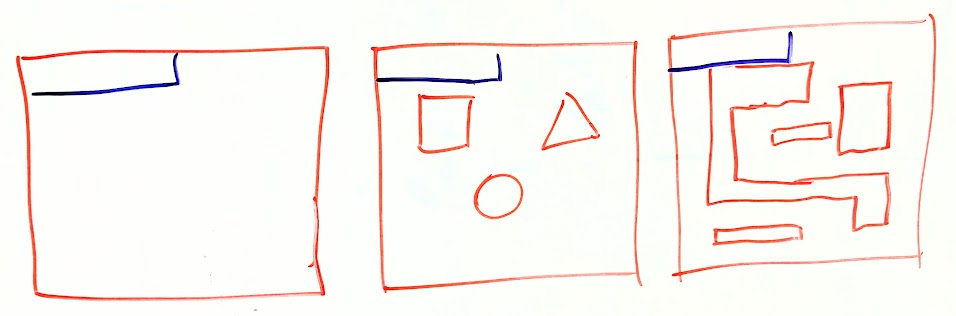
\includegraphics[width=0.8\textwidth]{Images/Example Environments.jpg}
    \caption{Environments of varying complexity used for testing. Blue area indicates starting area of the swarm \incomplete{This image is obviously just a mock-up, I'll make a proper diagram later}}
    \label{fig:example environments}
    \end{figure}

\subsection{Algorithms for Comparison}



\subsection{Treatments}

\subsection{Data Collected}
The main data collection target for these simulations will be \textbf{time to explore the environment}. This will be split into sub-measurements (80\%, 95\% and 99\% coverage), as well as an overall exploration rate value in $m^2/s$ collected throughout the simulation. These values will give a clear picture of how the system performs throughout its runtime rather than simply how long complete coverage takes. This is advantageous as complete coverage time can vary wildly if a small amount of space (in a corner for example) is missed on the first pass, and faster but slightly less complete coverage can be acceptable trade-off depending on the scenario. In addition, several other non-goal metrics will be collected:

\paragraph{Messages passed and communication bandwidth} are crucial metrics when it comes to scalability of the system, as in many systems message passing bandwidth of a given agent will scale $O(N^2)$ where N is the number of agents. A scalable system should have a message passing bandwidth of $O(N)$ to allow for unlimited expansion.

\paragraph{Message passing distances} directly determine the amount of radio power required to send a message, and crucially this also scales with $O(D^2)$. Therefore, keeping distance low has a significant impact on required transmit power.

\paragraph{There's more...}


\newpage
\section{Results}

\begin{table}
\caption{Time to complete exploration (99\%)}\label{tab1}
\begin{tabular}{|l|l|l|l|}
\hline
Algorithm &  Open Environment & Simple Obstacles & Complex Environment\\
\hline
My Algo             & 82s  & ... & ...\\
Tran-like           & 91s  & ... & ...\\
Naive algo          & 120s & ... & ...\\
Theoretical optima  & 40s  & ... & ...\\
\hline
\end{tabular}
\end{table}

I'd describe the results here if I had any that weren't made up


Maybe I should just focus on the open or the simple environment for now, so I can stick to analysing scalability?

% ---=== Bibliography ===---

\bibliographystyle{splncs04}
\bibliography{Library}
\end{document}
